\section{Detektion von Snooker-Kugeln}
Im Folgenden wird die Detektion geprüft, indem die Genauigkeit der detektierten Kugelpositionen, die Performanz und die
Robustheit gegenüber Fremdkörpern, wie Armen und Händen des Spielers, im Bild untersucht wird.

\subsection{Detektionsgenauigkeit}
Zur Überprüfung der Genauigkeit der Kugeldetektion wurden 50 Testbilder von verschiedenen Spielständen
mit einer kalibrierten Kamera aufgenommen.
Die Positionen der Kugeln wurden auf den Bildern manuell bestimmt und in Pixelkoordinaten angegeben.
Die Pixelkoordinaten wurden anschliessend in Modellkoordinaten umgewandelt \cite{project2:pixel_to_model_coordinates}.
Diese Referenzdaten können mit dem Resultat des Detektionsalgorithmus verglichen werden,
indem dieser die Kugeln auf denselben Bildern detektiert, auf dieselbe Weise in Modellkoordinaten umwandelt und
die Positionen mit den Referenzdaten verglichen werden.
Die Distanzen zwischen den Kugelpositionen in den Referenzdaten und in der Detektion können
anschliessend statistisch ausgewertet werden.

Im Vergleich zur Vorarbeit \cite{project2:resultate} wurden annotierte Referenzdaten für die Auswertung verwendet, da
in dieser Arbeit nur der Detektionsalgorithmus für die Bestimmung der Pixelkoordinaten der Kugeln überarbeitet wurde, um
die Live-Detektion zu erlauben, siehe Kapitel \ref{kap:detektion}.
Der Algorithmus zur Umwandlung von Pixelkoordinaten zu Modellkoordinaten \cite{project2:pixel_to_model_coordinates} wurde nicht verändert.
Deshalb wurde hier auf eine Messung der physischen Position der Kugeln verzichtet und stattdessen mit annotierten Bildern gearbeitet.
Dafür konnten mehr Positionsdaten für die Auswertung gesammelt werden, als dies mit einer Messung zeitlich möglich gewesen wäre.

In den 50 Referenzbildern sind insgesamt 835 Kugelpositionen hinterlegt, in Tabelle \ref{tab:detektion_resultate_distanzen_stats}
sind einige statistische Kennzahlen aus diesem Vergleich aufgeführt. Der Median liegt bei ca. 2.33mm und 50\% der Detektionen
haben einen Positionsfehler zwischen ca. 0mm - 3.7mm.
Die maximale Abweichung zwischen Referenzdaten und Detektion liegt bei 8.35mm.

\begin{table}[ht]
    \rowcolors{1}{\seccolor!10}{\seccolor!10} % Rows with 10% of secondary color
    \begin{tabular}{ rrrrrr }
        \rowcolor{\seccolor!50}
        Anzahl Kugeln & Minimum & Unteres Quartil & Median & Oberes Quartil & Maximum\\
        835 & 0.000004mm & 0.000601mm & 2.329217mm & 3.680264mm & 8.3566mm
    \end{tabular}
    \caption{Statistische Zahlen zu den Distanzen zwischen den Kugelpositionen der Referenzdaten und den detektierten Kugelpositionen.}
    \label{tab:detektion_resultate_distanzen_stats}
\end{table}

% Pixel distance: count=624, min=0.000000, lower quartile=1.000000, median=1.414214, upper quartile=2.236068, max=5.099020
% Model distance: count=835, min=0.000004, lower quartile=0.000601, median=2.329217, upper quartile=3.680264, max=8.356600

In Abbildung \ref{fig:detection_results_bad_detections} sind die beiden grössten Detektionsfehler abgebildet.
Dabei handelt es sich um Fälle, wo die detektierte Pixelposition um bis zu 5 Pixel Abweichung gegenüber den Referenzdaten aufweist.
Aus diesen Abweichungen in Pixeln sind Abweichungen bis maximal 8.35mm entstanden.

\begin{figure}[h!]
    \centering
    \begin{subfigure}[t]{0.3\textwidth}
        \centering
        
\includegraphics[width=1.0\linewidth]{../common/04_results/resources/bad_detection_4_8.356600_5.099020.png}
        \caption{Detektionsfehler einer roten Kugel von 5 Pixel und 8.35mm}
        \label{fig:detection_results_bad_detection_1}
    \end{subfigure}
    \begin{subfigure}[t]{0.3\textwidth}
        \centering
        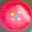
\includegraphics[width=1.0\linewidth]{../common/04_results/resources/bad_detection_5_7.727108_4.472136.png}
        \caption{Detektionsfehler einer pinken Kugel von 4.47 Pixel und 7.72mm}
        \label{fig:detection_results_bad_detection_2}
    \end{subfigure}
    \caption{
        Die grössten festgestellten Fehler in der Positionsdetektion. Gelb ist die detektierte Kugelposition, türkis die Position aus den Referenzdaten.
        Ein gewisser Fehler in den Referenzdaten ist bei diesen Positionen nicht auszuschliessen.
    }
    \label{fig:detection_results_bad_detections}
\end{figure}

In Tabelle \ref{tab:detektion_resultate_distanzen_stats_pro_kugelfarbe} wurden die Positionsfehler der Detektion
gegenüber den Referenzdaten pro Kugelfarbe ausgewertet.
Es wurden lediglich 32 der 50 Referenzbilder verwendet, da bei den anderen die korrekten Farben der Kugeln nicht hinterlegt wurden.
Es gibt bei den meisten Kugelfarben keine grossen Unterschiede zu den Zahlen in Tabelle \ref{tab:detektion_resultate_distanzen_stats}.
Lediglich bei den Kugelfarben gelb und grün liegt der Median tiefer als bei allen anderen Kugelfarben.

\begin{table}[ht]
    \rowcolors{1}{\seccolor!10}{\seccolor!10} % Rows with 10% of secondary color
    \begin{tabular}{ lrrrrrrr }
        \rowcolor{\seccolor!50}
        Kugelfarbe & Anzahl Kugeln & Minimum & Unteres Quartil & Median & Oberes Quartil & Maximum\\
        BROWN & 32 & 0.000153mm & 1.682379mm & 2.454655mm & 3.740010mm & 5.395337mm \\
        PINK & 32 & 0.000076mm & 1.678389mm & 2.338619mm & 3.422637mm & 7.727108mm \\
        RED & 224 & 0.000004mm & 1.672397mm & 2.358258mm & 3.659417mm & 8.356600mm \\
        BLACK & 32 & 0.000218mm & 1.685366mm & 2.377796mm & 3.794632mm & 4.688987mm \\
        YELLOW & 32 & 0.000011mm & 1.685552mm & 1.716131mm & 3.393303mm & 5.378226mm \\
        WHITE & 32 & 0.000086mm & 1.677719mm & 2.357014mm & 3.775538mm & 5.394620mm \\
        BLUE & 32 & 0.000071mm & 1.684771mm & 2.351218mm & 3.419713mm & 5.391995mm \\
        GREEN & 32 & 0.000041mm & 0.000356mm & 1.707863mm & 3.703774mm & 7.039578mm
    \end{tabular}
    \caption{Statistische Zahlen zu den Distanzen zwischen den Kugelpositionen der Referenzdaten und den detektierten Kugelpositionen pro Kugelfarbe.}
    \label{tab:detektion_resultate_distanzen_stats_pro_kugelfarbe}
\end{table}

Die verwendete Vergleichsmethode enthält an sich bereits einen Fehlerbereich, welcher der Auflösung des Bildes geschuldet ist.
Eine genaue Beschreibung ist in \cite{project2:fehler_grundwahrheit} enthalten, hier werden die wichtigsten Erkenntnisse
erneut aufgeführt.
Die Ausmasse des Spielbereichs des Billardtisches betragen 1881mm mal 943mm, die Auflösung des Bildes beträgt 1280x720 Pixel.
Der Spielbereich füllt nicht die gesamte Bildauflösung, sondern lediglich 1118x565 Pixel.
Ein einzelnes Pixel des Bildes entspricht damit einer Fläche von 1.681mm mal 1.668mm.
Der Detektionsalgorithmus detektiert die Kugelpositionen subpixelgenau.
Die maximale Abweichung unter der Annahme, dass das korrekte Pixel in den Referenzdaten angegeben wurde, beträgt 1.18406mm.

Die Annahme, dass in den Referenzdaten das korrekte Pixel angegeben wurde, ist selbstverständlich höchst unwahrscheinlich.
In Abbildung \ref{fig:detektion_resultate_min_max_fehler_referenzdaten} sind verschiedene Fälle aufgeführt,
um eine Aussage darüber zu machen, wie sich ein Fehler in den Referenzdaten auf deren Genauigkeit auswirkt.

\begin{figure}[h!]
    \begin{center}
        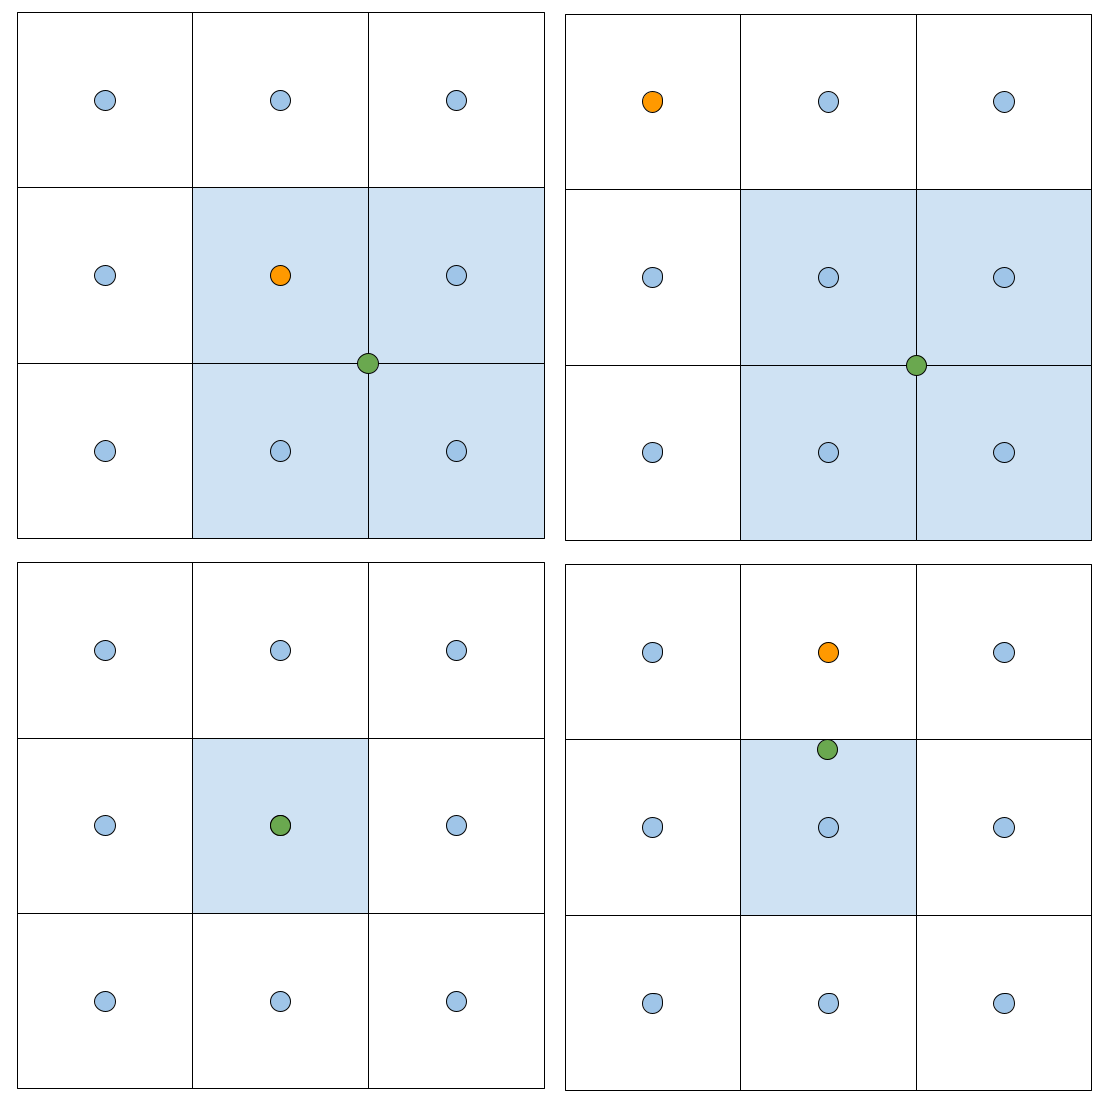
\includegraphics[width=0.5\linewidth]{../common/04_results/resources/detektion_min_und_max_fehler.png}
    \end{center}
    \caption{
        Extremsituationen zum Vergleich der Referenzposition und der wahren Position des Kugelmittelpunktes.
        Abgebildet ist ein Bildausschnitt mit 9 Pixeln. Die blauen Punkte sind die Pixelzentren, grün ist die wahre Position (subpixelgenau), orange ist die Referenzposition aus den Referenzdaten.
        Die Pixel rund um die wahre Position sind blau hinterlegt.
        Oben-Links: Der maximale Fehler ist eine halbe Pixeldiagonale, wenn die wahre Position zwischen vier Pixeln liegt und die Referenzposition einem der Pixel rund um die tatsächliche Position entspricht.
        Unten-Links: Der minimale Fehler ist $0$, wenn die wahre Position genau dem Pixelzentrum entspricht und dieses Pixel in den Referenzdaten ausgewählt wurde.
        Oben-Rechts: Der maximale Fehler ist 1.5 Pixeldiagonalen, wenn die wahre Position zwischen vier Pixeln liegt und die Referenzposition um ein Pixel daneben ist.
        Unten-Rechts: Der minimale Fehler ist eine halbe Pixelbreite/-höhe, wenn die wahre Position innerhalb des zentralen Pixels liegt und die Referenzposition um ein Pixel daneben ist.
    }
    \label{fig:detektion_resultate_min_max_fehler_referenzdaten}
\end{figure}

In Abschnitt \ref{kap:tracking} wurde beschrieben, dass in der Live-Detektion eine Stabilisierung der detektierten Positionen
über die Zeit durchgeführt wird.
In diesem Kapitel wurden nur Bilder für den Vergleich zwischen Detektion und Realität verwendet, wodurch es sich um Momentaufnahmen handelt.
Es kann sein, dass die Stabilisierung in gewissen Fällen die detektierten Positionen verbessert,
weil Positionsfehler in einzelnen Bildern geglättet werden.

\subsection{Performanz der Live-Detektion}
Die Performanz der Detektion ist für das Tracking und die Anzeige der Kugelpositionen in Echtzeit relevant.
Zur Messung wurde die Detektion 50-mal abwechselnd auf 24 Testbildern ausgeführt und die benötigte Zeit gemessen.
Dadurch wurden $50 \cdot 24 = 1200$ Detektionen ausgeführt.
Ausgeführt wurde dieser Test auf einem vierjährigen Laptop vom Modell Acer Aspire V 15 Nitro mit
einem Intel(R) Core(TM) i7-7700HQ CPU @ 2.80GHz und 16GB RAM.

Aufgrund dieses Tests konnte die durchschnittliche Dauer eines Detektionsdurchlaufs berechnet werden.
Diese beträgt 43.8ms und entspricht damit einer Framerate von 22.8 fps (frames per second).
Mit der aktuell eingesetzten Kamera, einer Intel RealSense D435 \cite{project2:aufbau}, kann mit der verwendeten Auflösung eine Framerate von
30 fps erreicht werden.
Mit dieser Performanz werden dementsprechend einzelne Frames übersprungen.
Die erreichte Performanz reicht allerdings aus, um Kugeln bei mittleren Geschwindigkeiten mit einer kleinen Verzögerung
zu verfolgen, siehe Abbildung \ref{fig:detection_delay}.

\begin{figure}[h!]
    \begin{center}
        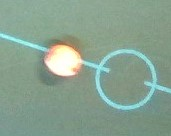
\includegraphics[width=0.4\linewidth]{../common/04_results/resources/detection_delay.jpg}
    \end{center}
    \caption{
        Sichtbare Verzögerung in der Detektion (vergrösserter Bildausschnitt).
        Die vergangene Zeit zwischen Bildaufnahme und Anzeige des Kreises um die detektierte Kugelposition herum ist zu gross,
        um die rollende Kugel perfekt zu verfolgen.
    }
    \label{fig:detection_delay}
\end{figure}

\subsection{Fehldetektionen an Armen und Händen}\label{kap:detektion_arme_haende}
Ein Problem der Live-Detektion ist, dass wenn ein Spieler mit der Hand in das Bild greift, um u.a. einen Stoss
durchzuführen, dann werden bei der Hand ebenfalls Kugeln detektiert, siehe Abbildung \ref{fig:detection_hand_problem}.
Dies ist darauf zurückzuführen, dass die Detektion eine Segmentierung des HSV-Farbraumes durchführt \cite{project2:snooker_detection}
und anschliessend darauf den Circle Hough transform \cite{wiki:circle_hough} ausführt.
Dadurch werden Kleider oder Haut ebenfalls als Bereiche erkannt, wo eine Kugel sein könnte.
Der Circle Hough transform findet anschliessend aufgrund von Kanten in diesen Bereichen Kreise,
welche dann als detektierte Kugeln übernommen werden.

\begin{figure}[h!]
    \begin{center}
        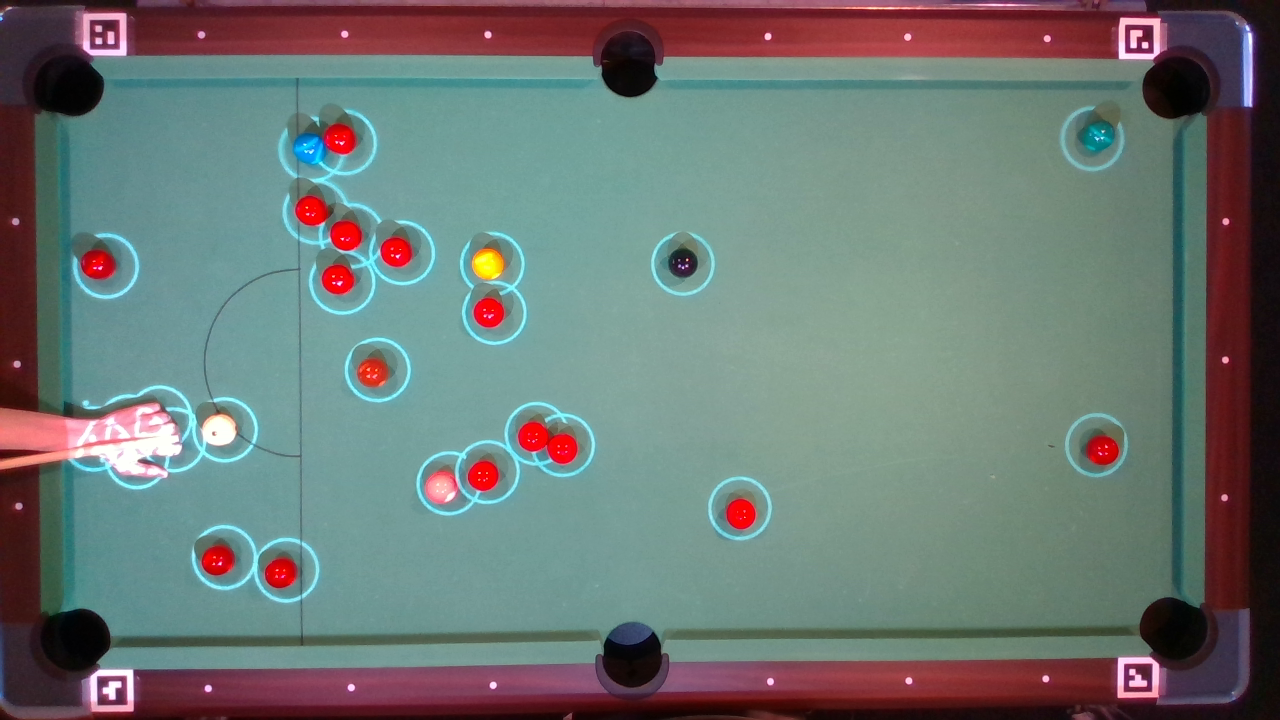
\includegraphics[width=0.8\linewidth]{../common/04_results/resources/detektierte_kugeln_auf_der_hand.png}
    \end{center}
    \caption{Fälschlich detektierte Kugeln auf der Hand}
    \label{fig:detection_hand_problem}
\end{figure}

Sofern die Arme und Hände des Spielers segmentiert werden könnten, wäre es möglich diese Fehler in der Detektion zu verhindern.
Dazu würden die segmentierten Regionen, wo eine Hand oder ein Arm abgebildet ist, in der Detektion ignoriert.
Diese Segmentation ist allerdings schwierig durchzuführen, da diese stark von Hautfarbe und Bekleidung abhängt.
Es wäre hier denkbar, ein vortrainiertes neuronales Netzwerk zu verwenden, welches eine Handsegmentation oder -detektion machen kann.

Die detektierten Kreise bei Armen und Händen sind mehrheitlich aus kosmetischen Gründen störend und könnten den Spieler ablenken.
Eine Suche sollte zum Zeitpunkt, da der Spieler gerade dabei ist, einen Stoss auszuführen, nicht durchgeführt werden.
Daher sind diese Fehldetektionen für die Suche irrelevant.
